\documentclass{article}

\usepackage{geometry}
\usepackage{xeCJK}
\usepackage{minted}
\usepackage[colorlinks,linkcolor=blue]{hyperref}
\usepackage{amsmath}
\usepackage{tikz}

% 设置页大小和页边距,或者scale=0.8
\geometry{a4paper,left=3.18cm,right=3.18cm,top=2.54cm,bottom=2.54cm}
% 声明分区,等宽字体:制表符号,等宽空格,ASCII,箭头字符
\xeCJKDeclareSubCJKBlock{MonoFont}{ "2500 -> "257F, "2002, "01 -> "F0, "2190 -> "21FF }
% 中文默认没有斜体和粗体格式,开启伪斜体和指定黑体;MonoFont分区指定字体为等宽字体Menlo
\setCJKmainfont[AutoFakeSlant, BoldFont=SimHei, MonoFont=Menlo]{SimSun}
% 全局设置代码样式,空格替换成英文等宽的字符0x2002
\setminted[java]{linenos, showspaces, space=\char"2002, fontsize=\small}

\begin{document}
\section{基础}
  \subsection{最大公约数}
  辗转相除法:
  \begin{enumerate}
    \item p和q为两个非负整数,且不同时为0;
    \item q为0时,则p为最大公约数;
    \item p \% q 余数为r;如果r为0,则结果为q;
    \item 如果r不为0;则p = q;q = r;继续上一步骤(\textbf{与余数辗转相除})
  \end{enumerate}

  \inputminted{java}{src/chapter01/GCD.java}

  \subsection{抽象数据类型(ADT)}
  抽象数据类型(Abstract Data Type,ADT),对算法结构的抽象,简化描述抽象的算法。

  \subsection{二分查找}
  \begin{enumerate}
    \item 已经排序的元素列表;以及待查询的目标元素;查询时,每次减半;
    \item 列表中间元素大于目标元素,则继续查询\textbf{[low, mid - 1]};
    \item 列表中间元素小于目标元素,则继续查询\textbf{[mid + 1, high]};
    \item 直到中间元素与目标元素相等,返回mid;或者low > high,返回-1。
  \end{enumerate}

  \inputminted{java}{src/chapter01/BinarySearch.java}

  \subsection{算术表达式运算}
  目前支持+、-、*、/运算符,参考:\href{http://faculty.cs.niu.edu/~hutchins/csci241/eval.htm}{算法描述} 。
  \begin{enumerate}
    \item 数值入栈,左括号入栈;
    \item 操作符号,如果操作符栈不为空,操作符栈顶符号不为左括号,且栈顶符号优先级 $\geq$ 当前扫描的符号,循环计算双栈;每次将结果压入操作数栈;最后压入当前操作符到栈中;
    \item 右括号,循环计算双栈,直到操作符栈为空,或达到左符号;每次计算的结果重新压入操作数栈;
    \item 最后操作符栈不为空,继续循环计算。
  \end{enumerate}

  \inputminted{java}{src/chapter01/ArithmeticExpression.java}

  \subsection{定容栈}
  固定大小的栈;如果需要扩容,提供resize方法,在push方法中检测是否需要扩容,然后调用resize方法;可以创建更大的数组,然后复制到新的数组中。

  \inputminted{java}{src/chapter01/FixedCapacityStack.java}

  \subsection{栈的链表实现}
  链表实现的栈没有限制容量。

  \inputminted{java}{src/chapter01/LinkedStack.java}

  \subsection{队列的链表实现}

  \inputminted{java}{src/chapter01/LinkedQueue.java}

  \subsection{背包}
  背包和栈类似,把push替换成add,然后移除pop;背包只添加元素,以及遍历元素。栈和队列也可以实现Iterator接口。

  \inputminted{java}{src/chapter01/Bag.java}

  \subsection{算法分析}
  \subsubsection{增长数量级分类}

  \begin{enumerate}
    \item 常数级别:$1$
    \item 对数级别:$\log N$
    \item 线性级别:$N$
    \item 线性对数级别:$N * \log N$
    \item 平方级别:$N^2$
    \item 立方级别:$N^3$
    \item 指数级别:$2^N$
  \end{enumerate}

  \subsubsection{2-sum}
  \inputminted{java}{src/chapter01/TwoSum.java}

  \subsubsection{3-sum}
  \inputminted{java}{src/chapter01/ThreeSum.java}

  \subsubsection{下界}
  在2-sum和3-sum例子中,是否能找到更优的算法,为算法在最坏的情况下的运行时间给出一个下界。

  \subsubsection{倍率实验}
  每次增加一倍输入规模,然后计算问题解决所需的时间,以此来预测任意问题的运行时间的增长数量级。

  \subsection{union-find算法}
  \subsubsection{动态连通性}
  输入一系列无序对,一对无序对p和q的关系为对等关系,即相连:
  \begin{enumerate}
    \item 自反性:p和p是相连,q和q是相连;
    \item 对称性:如果p和q相连,那么q和p相连;
    \item 传递性:如果p和q相连,q和r相连,那么p和r相连;
  \end{enumerate}
  对等关系能够将对象分为多个等价类;对象p和q相连时,那么p和q为同一分类。

  \subsubsection{Quick-Find实现}
  find()常数级别;union()线性级别,如果N个连通分量全部合并,则为平方级别。
  \inputminted{java}{src/chapter01/QuickFind.java}

  \subsubsection{Quick-Union实现}
  find()最坏情况下线性级别;union()最坏情况下线性级别,如果N个连通分量全部合并,则为平方级别;
  Quick-Union实现方式不一定比Quick-Find方式快,这取决于输入样本,取决于树的高度。
  \inputminted{java}{src/chapter01/QuickUnion.java}

  \subsubsection{加权Quick-Union实现}
  find()、union()、connected()最坏情况下也是对数级别。
  \inputminted{java}{src/chapter01/WeightedQuickUnion.java}

  \section{排序}
  \subsection{交换排序}
    \subsubsection{冒泡排序}
    思路:从底部开始,两两比较,最小的上浮冒泡
    \\[10pt] 分析:稳定;平均时间$N^2$;最好时间$N$;最坏时间$N^2$
    \inputminted{java}{src/chapter02/BubbleSort.java}

    \subsubsection{快速排序}
    思路:
    \begin{enumerate}
      \item 分区:基准值的插入位置;
      \begin{enumerate}
        \item 随机获取基准值;基准值与尾部元素交换;
        \item 循环左右扫描,直到low与height相遇;
        \item 左边向右边方向一直扫描,直到比pivot大,low插入到height位置;
        \item 右边向左边方向一直扫描,直到比pivot小,height插入到low位置;
        \item low = height,pivot插入到low与height重叠的位置;
        \item 返回插入位置。
      \end{enumerate}
      \item 分治:基准值两边重复快速排序。
    \end{enumerate}
    分析:不稳定;平均时间$N \log N$;最好时间$N \log N$;最坏时间$N^2$

    \inputminted{java}{src/chapter02/QuickSort.java}

  \subsection{选择排序}
    \subsubsection{直接选择排序}
    思路:
    \begin{enumerate}
      \item 数组组成:已排序部分 + 待排序部分;
      \item 每轮选取最小的值,移至待排序头部;
      \item 完成该轮的排序,继续后面的待排序部分。
    \end{enumerate}
    分析:不稳定;平均时间$N^2$;最好时间$N^2$;最坏时间$N^2$

    \inputminted{java}{src/chapter02/SelectionSort.java}

    \subsubsection{堆排序}
    思路:
    \begin{enumerate}
      \item 将数组建立成大根堆;
      \item 第一个肯定是最大的,将第一个与最后一个交换;
      \item 继续将[0, n - 2]个元素建立成大根堆;
      \item 继续第2步骤,直到元素从右往左,从大到小排序好。
    \end{enumerate}
    分析:不稳定;平均时间$N \log N$;最好时间$N \log N$;最坏时间$N \log N$

    \inputminted{java}{src/chapter02/HeapSort.java}

  \subsection{插入排序}
    \subsubsection{直接插入排序}
    思路:类似打牌时采用的排序方式
    \begin{enumerate}
      \item 分有序区和无序区;
      \item 将无序区中的第一个元素插入到有序区的适合位置中。(在有序区中: 从右往左扫描)
    \end{enumerate}
    分析:稳定;平均时间$N^2$;最好时间$N$;最坏时间$N^2$

    \inputminted{java}{src/chapter02/HeapSort.java}

    \subsubsection{希尔排序}
    思路:按一定增量的直接插入算法
    \begin{enumerate}
      \item 步长每次减半,直到步长为1,变成普通插入排序;
      \item 从gap开始,从左往右,从上到下,直到数组尾部,直接插入排序
    \end{enumerate}
    分析:不稳定;平均时间,取决于gap的选取;最好时间$N \log N$;最坏时间$N^2$(选取最坏的gap)、$N {\log}^2 N$(选取最优的gap)

    \inputminted{java}{src/chapter02/ShellSort.java}

  \subsection{归并排序}
    \subsubsection{归并排序}
    思路:分治思想
    \begin{enumerate}
      \item 将数组分成2半;
      \item 数组左边部分继续分治,归并排好序;
      \item 数组右边部分继续分治,归并排好序;
      \item 直到分成数组只有一个元素;
      \item 然后将两个排好序的数组归并。
    \end{enumerate}
    分析:稳定;平均时间$N \log N$;最好时间$N \log N$;最坏时间$N \log N$

    \inputminted{java}{src/chapter02/MergeSort.java}

  \section{查找}
    \subsection{顺序查找}
      条件:无序或有序;
      \\[10pt] 思路:遍历元素,待查找目标元素与数组中每个元素比较,该算法简单,不提供代码。
      \\[10pt] 分析:平均和最坏时间复杂都是$N$
    \subsection{二分查找}
      条件:有序;
      \\[10pt] 思路:依次与区间中间的值比较,如果相等,则返回位置,否则区间减半,继续比较直到找到或条件区间不合理返回-1。
      \begin{enumerate}
        \item 条件:合理区间:$low <= height$;
        \item 比较:$data[mid] ==  target, \; return \; mid$;
        \item 比较:$data[mid] < target, \; low = mid + 1$;
        \item 比较:$data[mid] > target, \; height = mid - 1$;
        \item 结束循环:返回-1。
      \end{enumerate}
      分析:最坏和平均都是$\log N$
      \inputminted{java}{src/chapter03/BinarySearch.java}
    \subsection{插值查找}
      条件:有序;
      \\[10pt] 思路:类似二分查找,但插值查找的中间点通过预测来减少查找次数,如果数组元素具有线性排序,则可以通过线性插值来预测mid,如下图:

      \begin{figure}
        \centering
          % 插值搜索
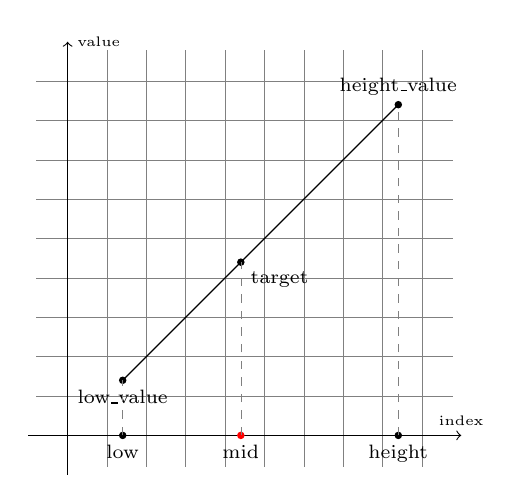
\begin{tikzpicture}
  \tikzstyle{every node}=[font=\scriptsize]

  \draw[step=.5cm,gray,very thin] (-0.4,-0.4) grid (4.9,4.9);
  \draw [->] (-0.5,0) -- (5,0);
  \node [above] at (5,0) {\tiny index};
  \draw [->] (0,-0.5) -- (0,5);
  \node [right] at (0,5) {\tiny value};
  \draw (0.7,0.7) -- (4.2,4.2);

  \draw[fill] (0.7,0.7) circle [radius=0.04];
  \node [below] at (0.7,0.7) {low\_value};
  \draw[fill] (0.7,0) circle [radius=0.04];
  \node [below] at (0.7,0) {low};

  \draw[fill] (2.2,2.2) circle [radius=0.04];
  \node [below right] at (2.2,2.2) {target};
  \draw[fill,red] (2.2,0) circle [radius=0.04];
  \node [below] at (2.2,0) {mid};

  \draw[fill] (4.2,4.2) circle [radius=0.04];
  \node [above] at (4.2,4.2) {height\_value};
  \draw[fill] (4.2,0) circle [radius=0.04];
  \node [below] at (4.2,0) {height};

  \draw[dashed,gray,very thin] (0.7,0) -- (0.7,0.7);
  \draw[dashed,gray,very thin] (2.2,0) -- (2.2,2.2);
  \draw[dashed,gray,very thin] (4.2,0) -- (4.2,4.2);
\end{tikzpicture}

          \caption{interpolation}
          \label{interpolation}
      \end{figure}

      \begin{enumerate}
        \item 两点式:$\frac{y - y2}{y1 - y2} = \frac{x - x2}{x1 - x2}$;
        \item 代入low和height两点坐标,以及target,求得:\newline $mid = low + \frac{(target - data[low]) * (height - low)}{data[height] - data[low]}$;
        \item 条件:
          \begin{enumerate}
            \item $data[height] - data[low] \neq 0 \Rightarrow data[height] \neq data[low]$
            \item target在[data[low], data[height]]区间:\newline $data[low] <= target \; \&\& \; target <= data[height]$
          \end{enumerate}
        \item 比较:$data[mid] ==  target, \; return \; mid$;
        \item 比较:$data[mid] < target, \; low = mid + 1$;
        \item 比较:$data[mid] > target, \; height = mid - 1$;
        \item 结束循环:返回-1。
      \end{enumerate}

      分析:如果元素分布均匀,呈线性分布,平均是$\log{(\log N)}$;最坏是当元素呈指数递增$O(N)$

      \inputminted{java}{src/chapter03/LinearInterpolationSearch.java}
    \subsection{Fibonacci查找}
    \subsection{树表查找}
    \subsection{分块查找}
    \subsection{哈希查找}

\end{document}
